\documentclass[12pt]{article}

% Packages
\usepackage[utf8]{inputenc}      % Encoding of the document
\usepackage{graphicx}            % For including images
\usepackage{amsmath, amssymb}    % Math packages
\usepackage{geometry}            % Page layout
\usepackage{hyperref}            % Hyperlinks
\usepackage{natbib}              % Bibliography
\usepackage{caption}             % Custom captions
\usepackage{subcaption}          % Subfigures
\usepackage{listings}            % Code listings
\usepackage{xcolor}              % Colors
\usepackage{biblatex}
\usepackage{tikz}                % Drawing
\usepackage{url}                 % URLs

% Bibliography file:
\addbibresource{bibliography.bib}

% To count pages after the index:
\pagenumbering{gobble}


% Page Layout
\geometry{
    a4paper,
    left=1in,
    right=1in,
    top=1in,
    bottom=1in,
}

% Hyperlink setup
\hypersetup{
    colorlinks=true,
    linkcolor=blue,
    filecolor=magenta,      
    urlcolor=cyan,
}

% Code Listing Style
\lstset{
    language=Python,
    basicstyle=\ttfamily\small,
    keywordstyle=\color{blue},
    commentstyle=\color{gray},
    stringstyle=\color{red},
    numbers=left,
    numberstyle=\tiny\color{gray},
    stepnumber=1,
    numbersep=10pt,
    backgroundcolor=\color{white},
    showspaces=false,
    showstringspaces=false,
    showtabs=false,
    frame=single,
    tabsize=4,
    captionpos=b,
    breaklines=true,
    breakatwhitespace=false,
    escapeinside={\%*}{*)},
}

% Title Information
\title{%
    \vspace{2in} % Adjust vertical space
    \textbf{Tackling the Traveling Salesman Problem with Genetic Algorithms}\\
    \vspace{2in}
}

\author{
    Mauro Vázquez Chas \\
    Dániel Mácsai
    \vspace{0.2in}
}

\date{2024. 11. 10}

\begin{document}

% Title Page
\maketitle
\thispagestyle{empty}

% Abstract
\begin{abstract}
    \noindent
    Abstract goes here.
\end{abstract}

\newpage

\tableofcontents
\newpage


%%%% start counting pages:
\pagenumbering{arabic}

%%%%%%%%%%%%%%%
\section{Introduction}
The Traveling Salesman Problem (TSP) is a classic combinatorial optimization problem that has been extensively studied in the field of mathematics and computer science. The problem is defined as follows: given a set of cities and the distances between them, the goal is to find the shortest possible route that visits each city exactly once and returns to the starting city. The TSP is an NP-hard problem, meaning that there is no known polynomial-time algorithm that can solve it exactly for all instances. In this sense, algorithms such us Genetic Algorithms (GAs) have been proposed as a way to find approximate solutions to the TSP.


\subsection{Background}
TODO: Provide background information on the topic, including relevant literature and the motivation behind the project.

\subsection{Objectives and scope}
\section{Objectives and Scope}

\subsection{Objectives}

The primary objective of this research is to investigate the effectiveness of Genetic Algorithms (GAs) in solving the Traveling Salesman Problem (TSP) and to identify optimal parameter configurations that lead to improved performance. Specifically, we aim to:

\begin{enumerate}
    \item \textbf{Implement} a GA framework to solve the TSP.
    \item \textbf{Experiment} with different genetic operators (crossover and mutation) and parent selection methods.
    \item \textbf{Tune} hyperparameters to optimize the GA's performance.
    \item \textbf{Evaluate} the performance of the GA on a benchmark TSP dataset.
    \item \textbf{Analyze} the impact of different parameter configurations on the solution quality and computational cost.
\end{enumerate}

\subsection{Scope}

The scope of this research is limited to the application of GAs to the TSP. We will focus on the following aspects:

\begin{itemize}
    \item \textbf{Problem Representation}: We will use a permutation-based representation to encode TSP solutions.
    \item \textbf{Genetic Operators}: We will implement and evaluate the performance of various crossover (e.g., Position-based Crossover, Order-based Crossover) and mutation (e.g., exchange mutation, insertion mutation, inversion mutation) operators.
    \item \textbf{Parent Selection}: We will explore different parent selection techniques, including random selection, roulette wheel selection, rank-based selection, and tournament selection.
    \item \textbf{Hyperparameter Tuning}: We will conduct experiments to determine the optimal values for hyperparameters such as population size, mutation rate, crossover rate, and number of generations.
    \item \textbf{Performance Evaluation}: We will evaluate the performance of the GA using the quality of the solutions obtained. 
\end{itemize}

We will not delve into more complex variations of the TSP, such as the Vehicle Routing Problem or the Capacitated Vehicle Routing Problem. Additionally, we will not explore other metaheuristic algorithms or hybrid approaches that combine GAs with other techniques.

%%%%%%%%%%%%%%%%%%%
\section{Methodology}
\subsection{Problem Representation}
In this work we employed the Pittsburgh view, where each individual in the population represents a complete solution to the TSP. The representation of the problem is a permutation of the cities, where each city is visited exactly once. For example, for a set of cities $\{1,2,3,4\}$, solution $\{1,3,2,4\}$ would represent the path in figure \ref{fig:tsp_example}.

\begin{figure}[h]
    \centering
    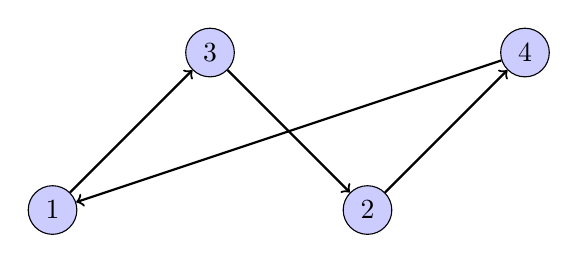
\begin{tikzpicture}
        % Define the nodes
        \node[circle, draw, fill=blue!20] (1) at (0, 0) {1};
        \node[circle, draw, fill=blue!20] (3) at (2, 2) {3};
        \node[circle, draw, fill=blue!20] (2) at (4, 0) {2};
        \node[circle, draw, fill=blue!20] (4) at (6, 2) {4};
        
        % Draw the arrows
        \draw[->, thick] (1) -- (3);
        \draw[->, thick] (3) -- (2);
        \draw[->, thick] (2) -- (4);
        \draw[->, thick] (4) -- (1);
    \end{tikzpicture}
    \caption{Path representation of a TSP solution with nodes 1, 3, 2, and 4.}
    \label{fig:tsp_example}
\end{figure}


We considered different approaches on the representation of each chromosome, either binary code or integer code. Using binary code, each solution would be a string of bits, with each city being a certain number of them. There are variations that use a different encoding mechanism, for example gray encoding. The integer code is a list of integers, where each city is represented by an integer. In the end, we decided to use integer code (called \textit{path representation} in \cite{Larranaga1999}), as it is more intuitive and in binary code, the number of bits used for each city could not be divided. This decision was also influenced by the research made in \cite{Larranaga1999}, where the authors explicitly state the following about binary code:
\begin{quote}
This representation might be useful for small problem instances of the TSP.
However, for larger problem instances the binary strings which represent
the tours become unmanageably large. Another disadvantage of the binary
representation is that the classical operators do not necessarily result in legal
offspring tours; repair algorithms would be necessary.
\end{quote}

In this sense, we are not doing what it is often called canonical or simple genetic algorithm (SGA) as it is described in \cite{Eiben2003}, where the representation is binary. It would be more accurate to say we are using Non-Canonical GAs with integer code representation for each permutation, as they are described in Chapter 17 of \cite{Back2000}. We think that this approach is more suitable for the TSP, as it allows for a more direct representation of the problem and avoids the need for additional repair mechanisms.

\subsection{An overview on Genetic Algorithms}
Genetic Algorithms are, perhaps, the most known evolutionary algorithm. They were pioneered by John Holland in the 1970s, and have since undergone extensive research and numerous adaptations. 

The traditional genetic algorithm, according to \cite{Eiben2003}, uses bit-string representation and works in the following way:
given a population of $\mu$ individuals, we perform the following steps for a certain number of generations:
\begin{enumerate}
    \item Select $\mu$ parents from the population, allowing duplicates
    \item Shuffle the intermediary population and apply crossover and mutation operators to create new individuals
    \item The intermediary population replaces the old population.
\end{enumerate}

The selection of the parents is often performed using a selection operator that often requires a fitness function evaluating the quality of the individuals. Classic operators for population modification include bit-flip mutation and one-point crossover.

\subsection{Parent Selection Methods}
Parent selection is a crucial step in the genetic algorithm, as it determines the genetic material that will be passed on to the next generation. In our case, we employed some of the most common mechanisms, according to the material proposed in the lectures \cite{Belanche2024}, and adapting them to the usage of the distance function instead of the fitness function (slightly different as we want to minimize it). The methods used were:
\begin{itemize}
    \item Random selection: parents are selected randomly from the population
    \item Roulette wheel selection: the probability of selecting an individual is proportional to its fitness (in our case, inversely proportional to the distance function)
    \item Rank roulette wheel selection: similar to the previous one, but the probability of selection is proportional to the rank of the individual (in our case, inversely proportional to the rank of the distance function)
    \item Tournament selection: a random subset of the population is selected, and the best individual from this subset is chosen as a parent. We used subsets of size 3 and 5.
\end{itemize}


\subsection{Crossover Techniques}

In genetic algorithms, crossover operators play a crucial role in combining the genetic information of two parent solutions to produce offspring. These techniques simulate the natural process of reproduction, where the genetic material of two parents is mixed to create offspring that inherit traits from both parents. The goal of the crossover operator is to generate new solutions that inherit the best features of the parents while maintaining diversity in the population. In this section, we describe two widely used crossover operators: the \textbf{Position-based Crossover (POS)} and \textbf{Order-based Crossover (OX1)} operators as these had the best result in \cite{Larranaga1999}.

\subsubsection{Position-based Crossover (POS)}

The \textbf{Position-based Crossover} (POS) operator is particularly useful when dealing with permutation-based problems, such as the \textbf{Traveling Salesman Problem (TSP)} or other problems where the solution involves a sequence of items or locations. In POS, the crossover is performed by selecting specific positions (or indices) from the parent chromosomes and transferring them to the offspring.

\paragraph{Implementation of POS Crossover:}

\begin{enumerate}
    \item \textbf{Input:} Two parent solutions, \texttt{Parent1} and \texttt{Parent2}, both represented as permutations of the same set of elements (e.g., cities in the TSP).
    \item \textbf{Process:}
    \begin{itemize}
        \item Randomly select a subset of positions (indices) from \texttt{Parent1}. These positions will be inherited by the offspring.
        \item Copy the elements from \texttt{Parent1} at the selected positions to the corresponding positions in the offspring.
        \item For the remaining positions, fill them with the elements from \texttt{Parent2}, ensuring that no element is repeated. This is done by copying the elements of \texttt{Parent2} that do not already exist in the offspring.
        \item We then repeat this process for the second offspring by swapping the roles of \texttt{Parent1} and \texttt{Parent2}.
    \end{itemize}
\end{enumerate}

\paragraph{Example:}

Suppose we have the following parents:
\[
\text{Parent1:} \ [4, 1, 3, 5, 2]
\quad \text{and} \quad \text{Parent2:} \ [2, 4, 1, 3, 5]
\]

A possible crossover operation could be:

\begin{enumerate}
    \item Randomly select a subset of positions from \texttt{Parent1}. For example, positions 1 and 3 (the corresponding elements are [4, 3]).
    \item Copy the elements at the selected positions from \texttt{Parent1} to the offspring. Now the partially filled offspring looks like this: \ [4, \_, 3, \_, \_].
    \item Fill the remaining positions with the elements from \texttt{Parent2} that are not already present in the offspring.
    \item Final \texttt{Offspring 1:} \ [4, 2, 3, 1, 5].
    \item For the second offspring, we use the same positions, the coresponing elements are [2, 1], so the offspring will look like this: \ [2, \_, 1, \_, \_].
    \item After filling it in from \texttt{Parent 1}, we end up with the final \texttt{Offspring 2:} \ [2, 4, 1, 3, 5].
\end{enumerate}



\paragraph{Role in Genetic Algorithm:}

POS crossover ensures that the offspring inherits a specific order of cities from \texttt{Parent1} while incorporating diversity by filling the remaining positions from \texttt{Parent2}. This technique is particularly effective for permutation-based problems as it preserves the relative ordering of elements while allowing diversity in the offspring population.

\subsubsection{Order-based Crossover (OX1)}

The \textbf{Order-based Crossover (OX1)} operator is another permutation-based crossover technique often used for solving combinatorial optimization problems. It is designed to preserve the relative ordering of elements from the parents while preventing duplicates in the offspring. OX1 works by selecting a subsequence of elements from one parent and then copying the remaining elements from the other parent in the same order they appear.

\paragraph{Implementation of OX1 Crossover:}

\begin{enumerate}
    \item \textbf{Input:} Two parent solutions, \texttt{Parent1} and \texttt{Parent2}, both represented as permutations.
    \item \textbf{Process:}
    \begin{itemize}
        \item Randomly select a subsequence of elements from \texttt{Parent1}. This subsequence will be retained in the offspring.
        \item For the remaining positions, copy the elements from \texttt{Parent2} in the order they appear, while ensuring that no element is duplicated in the offspring. This can be done by skipping over any element that is already present in the offspring.
        \item The second offspring is generated by swapping the roles of \texttt{Parent1} and \texttt{Parent2}, i.e., selecting a subsequence from \texttt{Parent2} and filling in the remaining positions with elements from \texttt{Parent1}.
    \end{itemize}
\end{enumerate}

\paragraph{Example:}

Given the parents:
\[
\text{Parent1:} \ [4, 1, 3, 5, 2]
\quad \text{and} \quad \text{Parent2:} \ [2, 4, 1, 3, 5]
\]

Suppose we randomly select a subsequence from \texttt{Parent1}, such as positions 2 to 4 (i.e., [1, 3, 5]). Now, the offspring will look like this:

\begin{enumerate}
    \item \texttt{Offspring 1(partially filled):} \ [\_, 1, 3, 5, \_] (copy positions 2 to 4 from \texttt{Parent1}).
    \item Copy the remaining elements from \texttt{Parent2} that are not yet in the offspring. The remaining elements from \texttt{Parent2} are [2, 4], which will fill the empty slots.
    \item Final \texttt{Offspring 1:} \ [2, 1, 3, 5, 4].
    \item For the second offspring, we select the same positions as before, the corresponding elements are [4, 1, 3], so the offspring will look like this: \ [\_, 4, 1, 3, \_], and after filling it, the final \texttt{Offspring 2} is \ [5, 4, 1, 3, 2].

\paragraph{Role in Genetic Algorithm:}

The \textbf{OX1 crossover} is particularly effective in maintaining the order of cities in the offspring, which is critical for problems like the TSP where the relative order of cities is important. By ensuring no duplicates and preserving order, OX1 allows for the effective exploration of the solution space while retaining useful genetic material from both parents. This leads to higher-quality offspring in the evolutionary process.

\subsubsection{Summary}

Both the \textbf{Position-based Crossover (POS)} and \textbf{Order-based Crossover (OX1)} operators are essential tools in solving permutation-based optimization problems like the TSP. These operators ensure that the offspring inherit useful traits from their parents while maintaining diversity and preventing duplicates. The role of these crossover techniques in a genetic algorithm is to generate high-quality solutions by combining the best features of the parent solutions and driving the algorithm towards the optimal solution. We see that basically the POS operator is a more general version of the OX1 operator, as it allows for more flexibility in the selection of the subsequence to be inherited from the first parent. At this point it is not clear if allowing more generality will result in better solutions or not, we will have to test it.

\subsection{Mutation Operators}
The mutation operator is a crucial part of the genetic algorithm, as it introduces diversity into the population. For further details, we referred to \cite{Larranaga1999}. In the end, in our implementation, we used the following mutation operators:

\begin{itemize}
    \item \textbf{Exchange mutation}: two random cities are arbitrarily swapped in the chromosome
    \item \textbf{Insertion mutation}: a random city is removed and reinserted at another random position in the chromosom
    \item \textbf{Inversion Mutation (IVM)}: A subset of the chromosome (i.e., a segment of the tour) is reversed. This mutation is effective in localizing improvements by reversing part of the tour, which may reduce the total travel distance. The \textbf{Inversion Mutation Algorithm (IVM)} follows these steps:
    
    \begin{enumerate}
        \item \textbf{Select the random subset}: Two indices, $i$ and $j$, are selected randomly such that $i < j$. These indices define the boundaries of the subset to be inverted. We now remove this subset, and reverse it. 
        
        \item \textbf{Replace the original segment}: The reversed segment is placed back into the chromosome into a randomly chosen position. 
    \end{enumerate}

    \noindent This mutation operator is effective in the \textbf{Travelling Salesman Problem (TSP)} because it can significantly alter the tour by reversing part of the path, which could potentially reduce the total travel distance. It is particularly useful when the cities in the selected subset are in an order that is suboptimal, as reversing them can yield better results.
\end{itemize}


Each of these mutation techniques introduces diversity into the population, ensuring that the genetic algorithm does not get stuck in local optima and can continue to evolve towards better solutions.


\subsection{Elitism}
Elitism is a mechanism that ensures that the best individuals from the current population are passed on to the next generation. This helps maintain the best solutions found so far and prevents the degradation of chromosome quality. In our implementation, we considered GA configurations without elitism and with elitism, both keeping the best individual and the three best individuals from the previous generation.

\subsection{Other Considered Approaches}
\subsubsection{Fitness Function}
As we already noted, we employed the total distance of the path as the value to minimize. However, the common approach would be to use a fitness function, where better chromosomes have higher values. In this sense, we could have used any monotonic decreasing function of the distance, for example, the reciprocal of the distance or a decaying exponential function. This would have allowed us to use the classic selection operators without modifications. However, we decided to use the distance directly, as it is more intuitive and straightforward.

\subsubsection{Population Replacement}
In this work we used a generational approach, where the entire population is replaced at each generation $(\mu,\lambda)$, with  $\mu=\lambda$. However, we also considered a steady-state approach where only a subset of the population is replaced at each generation. Ultimately we decided not to do this, as it would have required a more complex implementation and in words of \cite{Eiben2003}: "It can also lead to premature convergece as the population tends to rapidly focus on the fittest member". 

A useful follow-up of this work would be to implement a steady-state approach by inverse tournament selection as it doesn't remove as much genetic diversity, due to its innate randomness.

Even though we described our implementation as $(\mu,\lambda), \mu=\lambda$, it could be seen as a $(\mu,\lambda), \mu>\lambda$ approach when we make use of elitism, as we keep the best individuals from the previous generation: $\mu=\lambda+\text{elitism}$.


\subsubsection{Population Initialization}
We evaluated different ways to initialize the population, including random initialization (the one we opted for) and heuristic initialization. This last one, refers to the usage of a heuristic algorithm to generate the initial population. This could be useful for large instances of the TSP, as it would provide a good starting point for the genetic algorithm. The practice is commented in Chapter 13 of \cite{Back2000}, where the authors also explore the hybridization of evolutionary strategies with domain specific knowledge and algorithms, highlighting the good results of the available literature.

However, we decided not to implement this, as it would require the usage of a heuristic algorithm and other techniques that are out of the scope of this work. Having said this, it would be interesting to further explore this.

\subsubsection{Other Operators}
TODO: Write about some options and the reasons why we didn't use them. (computational time of the grid search, etc.)

% Implementation
\section{Implementation}
\subsection{Dataset}
In this work, we consider a dataset of 29 cities from Bavaria, Germany. The dataset contains the coordinates of each city, as well as the distances between them (provided in a distance matrix). The dataset (called \textit{bays29.tsp}) is available at the following link: \url{http://comopt.ifi.uni-heidelberg.de/software/TSPLIB95/tsp/}

\subsection{Code Structure}
One of our main goals, was to create a flexible and modular implementation that allows for easy experimentation with different configurations and operators. To achieve this, we used Python as the main programming language, and we implemented the parent-selection methods, crossover operators, and mutation operators as separate modules. This design allows us to easily swap out different operators and configurations without changing the core logic of the genetic algorithm. Aside from this, the class that contains the genetic algorithm is also modular, allowing for easy extension and modification. All of these files, can be found in the \textit{src} folder of the project.

Another clear target of ours, was to code (almost) everything from scratch. For this reason, we only used the following libraries:
\begin{enumerate}
    \item \textit{numpy} for numerical operations and efficiency
    \item \textit{random} for random number generation
    \item \textit{matplotlib} for visualization
    \item \textit{typing} for type hints
    \item \textit{logging} for better debugging
    \item \textit{json} to save the results
    \item \textit{datetime} to save the results
    \item \textit{pandas} to deal with the results in a more structured way for the analysis
\end{enumerate}

To use all of these modules, we set up a jupyter notebook file \textit{tsp.ipynb} that contains the data reading function, the grid search function and most graph plotting cells (see \ref{fig:code_structure}). In this notebook, we also wrote a \textit{Usage Example} section, where we show how to use the genetic algorithm class and all of its parameters, although if more insight is needed, all the functions and classes are documented in their respective docstrings.

\begin{figure}
    \centering
    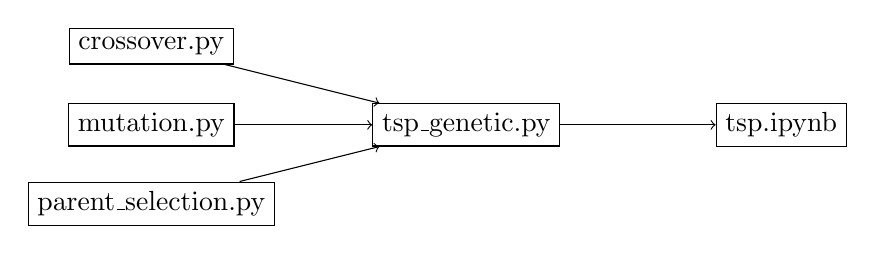
\begin{tikzpicture}[node distance=1cm, auto]
        % Nodes
        \node (crossover) [draw, rectangle] {crossover.py};
        \node (mutation) [draw, rectangle, below of=crossover] {mutation.py};
        \node (parent_selection) [draw, rectangle, below of=mutation] {parent\_selection.py};
        \node (tsp_genetic) [draw, rectangle, right of=mutation, node distance=4cm] {tsp\_genetic.py};
        \node (tsp_notebook) [draw, rectangle, right of=tsp_genetic, node distance=4cm] {tsp.ipynb};

        % Arrows
        \draw[->] (crossover) -- (tsp_genetic);
        \draw[->] (mutation) -- (tsp_genetic);
        \draw[->] (parent_selection) -- (tsp_genetic);
        \draw[->] (tsp_genetic) -- (tsp_notebook);
    \end{tikzpicture}
    \caption{Code Structure Diagram}
    \label{fig:code_structure}
\end{figure}

\subsubsection{Genetic Algorithm Class}
The core of our implementation is the \textit{tsp\_genetic.py} module, which contains the \textit{TSP\_Genetic} class. This class is responsible for running the genetic algorithm, given a set of parameters and operators. The class contains the following methods:
\begin{itemize}
    \item \textbf{\_\_init\_\_}: Initializes the genetic algorithm with the given hyperparameters. To see them, check \ref{annex:initparameters}.
    \item \textbf{run}: Runs the genetic algorithm for the specified initial population, cities and matrix of distances. \ref{annex:runparameters}
    \item \textbf{\_path\_distance}: Given a chromosome provides the total path distance.
    \item \textbf{path\_distance\_population}: Given a population, returns an array with the total path distance of each chromosome.
    \item \textbf{plot\_route}: Given a chromosome, plots its route.
\end{itemize}

\subsubsection{Crossover Class}
The \textit{crossover.py} module contains the \textit{Crossover} class, which is responsible for implementing the crossover operators. The class contains the following methods:
\begin{itemize}
    \item \textbf{POS}
    \item \textbf{OX1}
\end{itemize}
Each of the methods were coded so they could be tuned via hyperparameters, that can be introduced in the \textit{\_\_init\_\_} method of the class using the \textit{crossover\_call} parameter. For example, if we intend to use the "OX1" operator, setting its first and second cut value to the 4th positions counting from each end, we would introduce in the \textit{TSP\_Genetic} instantiation: \textit{crossover\_call = "(4, cities.shape[0] - 4)"}.
    


% Results
\section{Results}
\subsection{Experimental Setup}
Describe the experiments conducted, including parameters and datasets used.


The number of configurations considered was: 3240
The best chromosome found was: [11  8  4 25 28  2  1 20  0  7 26 22  6 24 18 10 21 13 16 17 14  3 19  9
 12 15 23 27  5]
The best distance found was: 2055.0
The best parameters were: {'population_size': 200, 'elitism': 1, 'generations': 200, 'm_rate': 0.1, 'c_rate': 1, 'select_parents': 'tournament_selection', 'crossover': 'POS', 'mutation': 'insertion', 'tournament_size': 5}


\subsection{Performance Analysis}
Present and analyze the results, using figures and tables as necessary.

\subsection{Discussion}
Interpret the results, discussing their implications and any observed patterns.

% Conclusion
\section{Conclusion}
\subsection{Summary}
Summarize the key findings and contributions of the project.

\subsection{Future Work}
Suggest potential areas for future research or improvements.

% References
\newpage
\printbibliography

% Appendix
\appendix
\section{Appendix: Hyperparameters}
\label{annex:parameters}
\subsection{\_\_init\_\_ Parameters}
\label{annex:initparameters}
\begin{itemize}
    \item \textbf{generations}: Number of generations to simulate.
    \item \textbf{print\_results}: Whether to print algorithm results.
    \item \textbf{print\_rate}: Frequency of progress printing.
    \item \textbf{m\_rate}: Mutation rate, probability of mutation in offspring.
    \item \textbf{c\_rate}: Crossover rate, probability of crossover between parent chromosomes..
    \item \textbf{select\_parents}: Parent selection method.
        \begin{itemize}
            \item \textbf{random\_selection}
            \item \textbf{roulette\_selection}
            \item \textbf{rank\_roulette\_selection}
            \item \textbf{tournament\_selection}
        \end{itemize}
    \item \textbf{tournament\_size}: Tournament size (just for tournament selection).
    \item \textbf{crossover}: Crossover method for parent chromosomes.
        \begin{itemize}
            \item \textbf{POS}
            \item \textbf{OX1}
        \end{itemize}
    \item \textbf{crossover\_call}: Arguments for the crossover method.
    \item \textbf{mutation}: Mutation method for offspring chromosomes.
        \begin{itemize}
            \item \textbf{exchange}
            \item \textbf{insertion}
            \item \textbf{IVM}
        \end{itemize}
    \item \textbf{elitism}: Number of best chromosomes retained in the next generation.
    \item \textbf{results\_path}: Path to save path\_distance statistics.
    \item \textbf{save\_results}: Save path\_distance statistics to a file.
\end{itemize}
\subsection{run Parameters}
\label{annex:runparameters}
\begin{itemize}
    \item \textbf{population}: Chromosomes in the initial population.
    \item \textbf{cities}: Matrix with the $(x,y)$ coordinates of each city.
    \item \textbf{distances}: Matrix of distances between cities.
\end{itemize}
\end{document}